% Options for packages loaded elsewhere
\PassOptionsToPackage{unicode}{hyperref}
\PassOptionsToPackage{hyphens}{url}
%
\documentclass[
]{article}
\usepackage{amsmath,amssymb}
\usepackage{iftex}
\ifPDFTeX
  \usepackage[T1]{fontenc}
  \usepackage[utf8]{inputenc}
  \usepackage{textcomp} % provide euro and other symbols
\else % if luatex or xetex
  \usepackage{unicode-math} % this also loads fontspec
  \defaultfontfeatures{Scale=MatchLowercase}
  \defaultfontfeatures[\rmfamily]{Ligatures=TeX,Scale=1}
\fi
\usepackage{lmodern}
\ifPDFTeX\else
  % xetex/luatex font selection
\fi
% Use upquote if available, for straight quotes in verbatim environments
\IfFileExists{upquote.sty}{\usepackage{upquote}}{}
\IfFileExists{microtype.sty}{% use microtype if available
  \usepackage[]{microtype}
  \UseMicrotypeSet[protrusion]{basicmath} % disable protrusion for tt fonts
}{}
\makeatletter
\@ifundefined{KOMAClassName}{% if non-KOMA class
  \IfFileExists{parskip.sty}{%
    \usepackage{parskip}
  }{% else
    \setlength{\parindent}{0pt}
    \setlength{\parskip}{6pt plus 2pt minus 1pt}}
}{% if KOMA class
  \KOMAoptions{parskip=half}}
\makeatother
\usepackage{xcolor}
\usepackage[margin=1in]{geometry}
\usepackage{longtable,booktabs,array}
\usepackage{calc} % for calculating minipage widths
% Correct order of tables after \paragraph or \subparagraph
\usepackage{etoolbox}
\makeatletter
\patchcmd\longtable{\par}{\if@noskipsec\mbox{}\fi\par}{}{}
\makeatother
% Allow footnotes in longtable head/foot
\IfFileExists{footnotehyper.sty}{\usepackage{footnotehyper}}{\usepackage{footnote}}
\makesavenoteenv{longtable}
\usepackage{graphicx}
\makeatletter
\def\maxwidth{\ifdim\Gin@nat@width>\linewidth\linewidth\else\Gin@nat@width\fi}
\def\maxheight{\ifdim\Gin@nat@height>\textheight\textheight\else\Gin@nat@height\fi}
\makeatother
% Scale images if necessary, so that they will not overflow the page
% margins by default, and it is still possible to overwrite the defaults
% using explicit options in \includegraphics[width, height, ...]{}
\setkeys{Gin}{width=\maxwidth,height=\maxheight,keepaspectratio}
% Set default figure placement to htbp
\makeatletter
\def\fps@figure{htbp}
\makeatother
\setlength{\emergencystretch}{3em} % prevent overfull lines
\providecommand{\tightlist}{%
  \setlength{\itemsep}{0pt}\setlength{\parskip}{0pt}}
\setcounter{secnumdepth}{-\maxdimen} % remove section numbering
\newenvironment{cols}[1][]{}{}

\newenvironment{col}[1]{\begin{minipage}{#1}\ignorespaces}{%
\end{minipage}
\ifhmode\unskip\fi
\aftergroup\useignorespacesandallpars}

\def\useignorespacesandallpars#1\ignorespaces\fi{%
#1\fi\ignorespacesandallpars}

\makeatletter
\def\ignorespacesandallpars{%
  \@ifnextchar\par
    {\expandafter\ignorespacesandallpars\@gobble}%
    {}%
}
\makeatother
\usepackage{subfig}
\ifLuaTeX
  \usepackage{selnolig}  % disable illegal ligatures
\fi
\IfFileExists{bookmark.sty}{\usepackage{bookmark}}{\usepackage{hyperref}}
\IfFileExists{xurl.sty}{\usepackage{xurl}}{} % add URL line breaks if available
\urlstyle{same}
\hypersetup{
  pdftitle={Diamonds analysis},
  pdfauthor={Oriade Simpson (s172084); Pietro Lombardo (s231756)},
  hidelinks,
  pdfcreator={LaTeX via pandoc}}

\title{Diamonds analysis}
\author{Oriade Simpson (s172084) \and Pietro Lombardo (s231756)}
\date{2023-09-05}

\begin{document}
\maketitle

\section{Contribution Table}\label{contribution-table}

\begin{center}\rule{0.5\linewidth}{0.5pt}\end{center}

\begin{longtable}[]{@{}lcc@{}}
\toprule\noalign{}
Task & Oriade & Pietro \\
\midrule\noalign{}
\endhead
\bottomrule\noalign{}
\endlastfoot
\textbf{Student ID} & s172084 & s231756 \\
------------- & -------------- & ------------- \\
Question 1 & x & \\
------------- & ------------- & ------------- \\
Question 2 & x & \\
------------- & ------------- & ------------- \\
Question 3 & & x \\
------------- & ------------- & ------------- \\
Question 4 & & x \\
------------- & ------------- & ------------- \\
Exam Prob 1 & & x \\
------------- & ------------- & ------------- \\
Exam Prob 2 & x & \\
------------- & ------------- & ------------- \\
Exam Prob 3 & x & \\
------------- & ------------- & ------------- \\
Exam Prob 4 & & x \\
------------- & ------------- & ------------- \\
Exam Prob 5 & & x \\
------------- & ------------- & ------------- \\
Exam Prob 6 & x & \\
\end{longtable}

\section{1) Description of the
dataset}\label{description-of-the-dataset}

\begin{itemize}
\tightlist
\item
  Explain what your data is about. I.e. what is the overall problem of
  interest?
\item
  Provide a reference to where you obtained the data.
\item
  Summarize previous analysis of the data. (i.e.~go through one or two
  of the original source papers and read what they did to the data and
  summarize their results).
\item
  You will be asked to apply (1) classification and (2) regression on
  your data in the next report. For now, we want you to consider how
  this should be done. Therefore: Explain, in the context of your
  problem of interest, what you hope to accomplish/learn from the data
  using these techniques?. Explain which attribute you wish to predict
  in the regression based on which other attributes? Which class label
  will you predict based on which other attributes in the classification
  task? If you need to transform the data in order to carry out these
  tasks, explain roughly how you plan to do this.
\end{itemize}

One of these tasks (1)--(5) is likely more relevant than the rest and
will be denoted the main machine learning aim in the following. The
purpose of the following questions, which asks you to describe/visualize
the data, is to allow you to reflect on the feasibility of this task.

\section{2) Explanation of the attributes of the
data}\label{explanation-of-the-attributes-of-the-data}

\begin{itemize}
\tightlist
\item
  Describe if the attributes are discrete/continuous,
  Nominal/Ordinal/Interval/ Ratio,
\item
  Give an account of whether there are data issues (i.e.~missing values
  or corrupted data) and describe them if so.
\item
  Include basic summary statistics of the attributes.
\end{itemize}

If your data set contains many similar attributes, you may restrict
yourself to describing a few representative features (apply common
sense).

\section{3) Data visualization}\label{data-visualization}

\subsection{Principal component
analysis}\label{principal-component-analysis}

The aim of the Principal Component Analysis (``PCA'' from now on), is to
simplify the problem dimension by reducing the number of variables which
explains the behavior of the diamonds' price.

The PCA requires the standardization of the attributes so that the
variability of each of them is comparable. But such operation cannot be
carried out for non-numeric values, like the three ordinal variables
\emph{cut}, \emph{color} and \emph{clarity}. For these reason they are
converted into ordinal numbers (from 1 to the upper level number)
according to their ranking.

After these operations, the dataset appears as below:

\begin{longtable}[]{@{}rrrrrrrrrr@{}}
\caption{Head of the diamonds dataset arranged for the
PCA}\tabularnewline
\toprule\noalign{}
carat & cut & color & clarity & depth & table & price & x & y & z \\
\midrule\noalign{}
\endfirsthead
\toprule\noalign{}
carat & cut & color & clarity & depth & table & price & x & y & z \\
\midrule\noalign{}
\endhead
\bottomrule\noalign{}
\endlastfoot
0.23 & 5 & 2 & 2 & 61.5 & 55 & 326 & 3.95 & 3.98 & 2.43 \\
0.21 & 4 & 2 & 3 & 59.8 & 61 & 326 & 3.89 & 3.84 & 2.31 \\
0.23 & 2 & 2 & 5 & 56.9 & 65 & 327 & 4.05 & 4.07 & 2.31 \\
0.29 & 4 & 6 & 4 & 62.4 & 58 & 334 & 4.20 & 4.23 & 2.63 \\
0.31 & 2 & 7 & 2 & 63.3 & 58 & 335 & 4.34 & 4.35 & 2.75 \\
0.24 & 3 & 7 & 6 & 62.8 & 57 & 336 & 3.94 & 3.96 & 2.48 \\
\end{longtable}

Now the dataset contains all numeric variables, so the next step is to
compare the standard deviations of each variable and check whether they
are different.

Below the standard deviations of the variables are shown:

\begin{verbatim}
##   carat     cut   color clarity   depth   table   price       x       y       z 
##    0.47    1.12    1.70    1.65    1.43    2.23 3989.44    1.12    1.14    0.71
\end{verbatim}

Since standard deviation of \emph{price} is some orders of magnitude
larger than the others, the dataset has to be standardized by
subtracting the mean and dividing by the standard deviation of the whole
set of observations of that variable.

\begin{cols}

\begin{col}{0.55\textwidth}
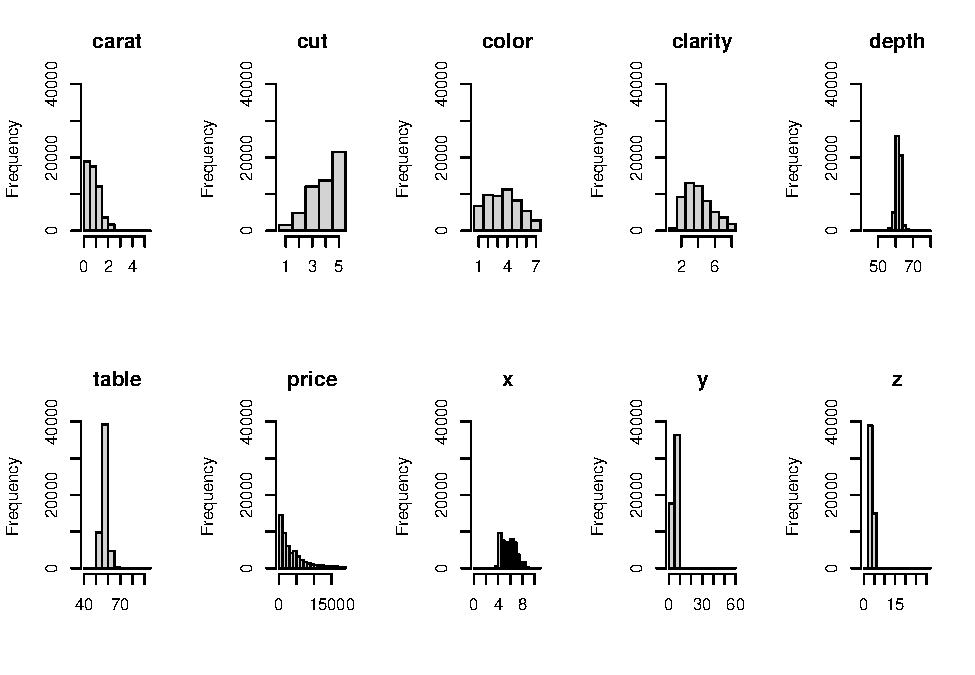
\includegraphics{Report_files/figure-latex/unnamed-chunk-4-1.pdf}

\end{col}

\begin{col}{0.05\textwidth}
~

\end{col}

\begin{col}{0.40\textwidth}
The new standardized dataset can be now used to perform the Singular
Value Decomposition (SVD), which gives rise to three different matrices:
\(U\), \(\Sigma\) and \(V^T\). By the extraction of the diagonal of the
matrix \(\Sigma\), it can be seen how much variance is explained by each
principal component. The cumulative explained variance should reach the
percentage of 90\% in order to describe properly the main features of
the dataset.

The figure on the left shows that the first 4 principal components
explain little less than the 90\% of variance

\end{col}

\end{cols}

\begin{cols}

\begin{col}{0.55\textwidth}
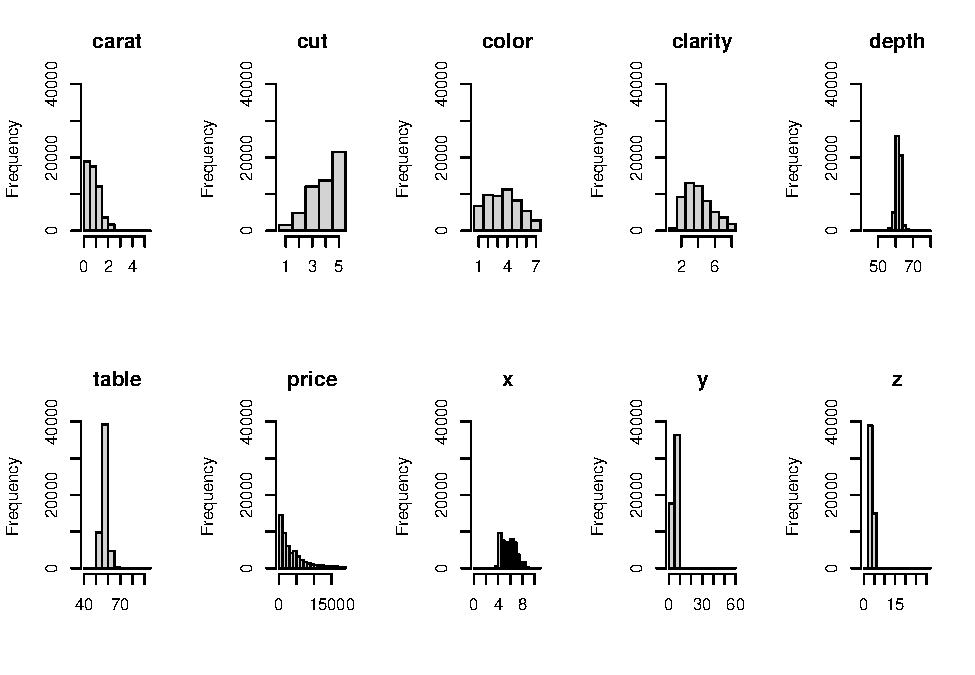
\includegraphics{Report_files/figure-latex/unnamed-chunk-5-1.pdf}

\end{col}

\begin{col}{0.05\textwidth}
~

\end{col}

\begin{col}{0.40\textwidth}
The matrix \(V^T\) contains the ten deca-dimensional vectors defining
the principal components (PCs). Focusing on the first four PCs, they
contains the weights associated to each of original component. The
figure on the left shows the valuea of the weights. It can be noticed
that the first PC mainly describes the dimensional quantities of the
diamonds (\emph{carat}, size in \emph{x}, \emph{y}, \emph{z}) and the
\emph{price}. It seems that these five characteristics alone explain
half of the variability of the diamonds. As for the second PC, it
focuses more on the quality characteristics (\emph{cut}, \emph{color},
\emph{clarity}) and on the \emph{table}.

\end{col}

\end{cols}

\begin{cols}

\begin{col}{0.55\textwidth}
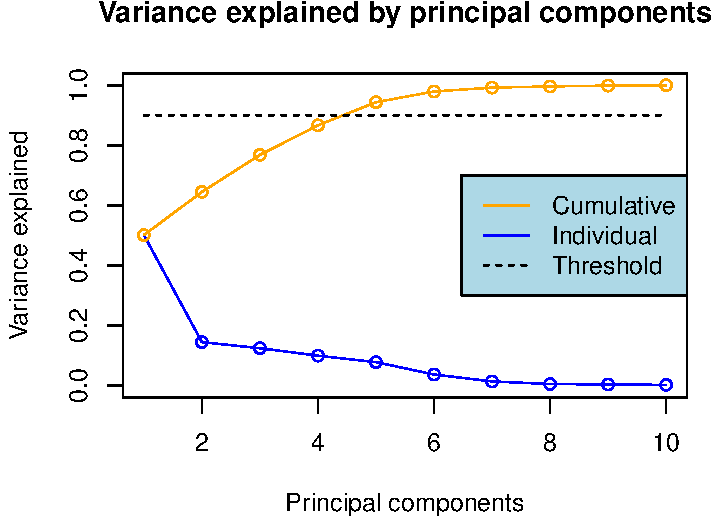
\includegraphics{Report_files/figure-latex/unnamed-chunk-6-1.pdf}

\end{col}

\begin{col}{0.05\textwidth}
~

\end{col}

\begin{col}{0.40\textwidth}
Unfortunately, it is impossible to represent data in a four-dimensional
space, so data are projected onto the bi-dimensional space defined by
the first two PCs. Coefficients can be projected in this space as well,
showing the directions followed by original attributes. It can clearly
be seen that the first PC is eastward oriented, so that it collects very
well the eastward attributes. Probably, the second PC is southward
directed so that it collects the southward attributes (with the plus
sign) and the northward \emph{table} attribute (with the minus sign)

\end{col}

\end{cols}

Data can be projected in all the possible bi-dimensional spaces defined
by each combination of two of the PCs. By projecting them, some
insteresting features can be observed, as shown by the four graphs
below.

\begin{itemize}
\tightlist
\item
  Variable \emph{cut} can assume five possible levels, so it is the
  easiest one to be visualized. The graph shows that \emph{cut} varies
  mostly in the direction of the second PC, so the \emph{cut} of
  diamonds strongly depends on their quality features (the better are
  \emph{color} and \emph{clarity}, the better will be the cut), and is
  less affected by the size (\emph{x}, \emph{y} and \emph{z}) and the
  \emph{carat} (weight);
\item
  variable \emph{price} is strongly asymmethrical towards low values,
  and it is very evident also in the graph where cold blue is
  predominant with respect to light blue. \emph{Price} strongly varies
  with the first PC, so it depends on quantity factors of diamonds (the
  bigger and heavier is the diamond, the more expensive will be) more
  than on quality ones;
\item
  variable \emph{carat} is very concentrated between 0 and 1 and
  widespread beyond 1. So, in order to have a better visualization, the
  graph below represent the logarithm of the \emph{carat}. It can be
  seen that it is correlated to the dimensional quantities explained by
  the first PC (the more expensive and bigger is the diamond, the
  heavier will be) more than quality ones;
\item
  variable \emph{color} has a better representation if data are
  projected onto the plan defined by the second and forth PCs. It can be
  seen that \emph{color} varies with the forth PC, so it is correlated
  with \emph{clarity}, \emph{cut} and \emph{table}.
\end{itemize}

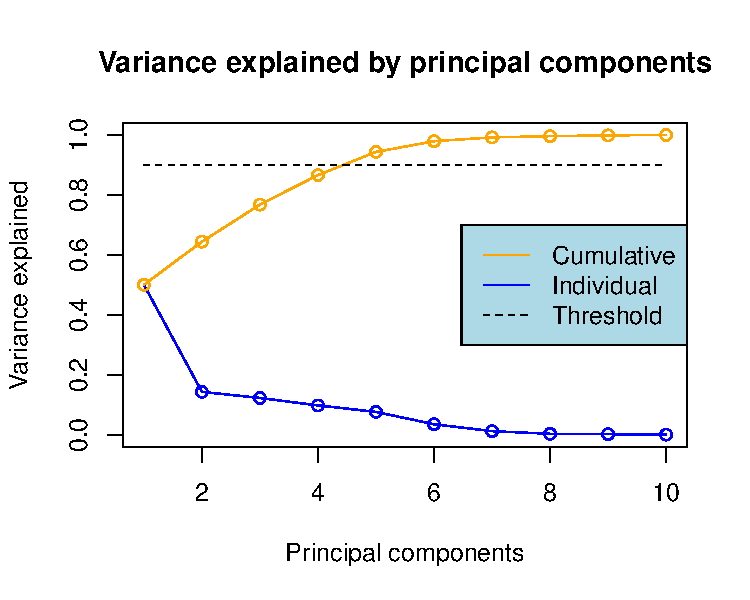
\includegraphics[width=0.5\linewidth]{Report_files/figure-latex/unnamed-chunk-7-1}
\includegraphics[width=0.5\linewidth]{Report_files/figure-latex/unnamed-chunk-7-2}
\includegraphics[width=0.5\linewidth]{Report_files/figure-latex/unnamed-chunk-7-3}
\includegraphics[width=0.5\linewidth]{Report_files/figure-latex/unnamed-chunk-7-4}

\section{4) Results: what data have
shown}\label{results-what-data-have-shown}

\end{document}
